% $Id: template.tex 11 2007-04-03 22:25:53Z jpeltier $

\documentclass{vgtc}                          % final (conference style)
%\documentclass[review]{vgtc}                 % review
%\documentclass[widereview]{vgtc}             % wide-spaced review
%\documentclass[preprint]{vgtc}               % preprint
%\documentclass[electronic]{vgtc}             % electronic version

%% Uncomment one of the lines above depending on where your paper is
%% in the conference process. ``review'' and ``widereview'' are for review
%% submission, ``preprint'' is for pre-publication, and the final version
%% doesn't use a specific qualifier. Further, ``electronic'' includes
%% hyperreferences for more convenient online viewing.

%% Please use one of the ``review'' options in combination with the
%% assigned online id (see below) ONLY if your paper uses a double blind
%% review process. Some conferences, like IEEE Vis and InfoVis, have NOT
%% in the past.

%% Figures should be in CMYK or Grey scale format, otherwise, colour
%% shifting may occur during the printing process.

%% These three lines bring in essential packages: ``mathptmx'' for Type 1
%% typefaces, ``graphicx'' for inclusion of EPS figures. and ``times''
%% for proper handling of the times font family.

\usepackage{mathptmx}
\usepackage{graphicx}
\usepackage{times}

\usepackage{algorithm}% http://ctan.org/pkg/algorithm
\usepackage{algpseudocode}% http://ctan.org/pkg/algorithmicx

\usepackage{url}

\usepackage{color}
\newcommand{\m}{\textcolor{red}}

\usepackage{multirow}
\usepackage{tabularx}

\usepackage{subfigure}
% \usepackage{subcaption}

\newcommand*{\WineMenuColor}{black}%
\newcommand*{\StartMenu}{\includegraphics[scale=0.2]{img/object_label.png}}%
\newcommand*{\WinMenu}[1]{
\StartMenu}

%\textcolor{red/blue/green/black/white/cyan/magenta/yellow}{text}

\usepackage{algpseudocode}


\algnewcommand{\IIf}[1]{\State\algorithmicif\ #1\ \algorithmicthen}
\algnewcommand{\EndIIf}{\unskip\ \algorithmicend\ \algorithmicif}

%\usepackage[demo]{graphicx}

%% We encourage the use of mathptmx for consistent usage of times font
%% throughout the proceedings. However, if you encounter conflicts
%% with other math-related packages, you may want to disable it.

%% If you are submitting a paper to a conference for review with a double
%% blind reviewing process, please replace the value ``0'' below with your
%% OnlineID. Otherwise, you may safely leave it at ``0''.
%\onlineid{2707}

%% declare the category of your paper, only shown in review mode
\vgtccategory{Research}

%% allow for this line if you want the electronic option to work properly
\vgtcinsertpkg

%% In preprint mode you may define your own headline.
%\preprinttext{To appear in an IEEE VGTC sponsored conference.}

%% Paper title.

\title{Unfolding the City: Exploring Mobility Patterns with Individual Characteristics}
%Interaction-On: Interaction Argument to Facilitate Visual Exploration on Web
%Filter+: Interaction Argument for Existing Web-based Visualizations

%% This is how authors are specified in the conference style

%% Author and Affiliation (single author).
%%\author{Roy G. Biv\thanks{e-mail: roy.g.biv@aol.com}}
%%\affiliation{\scriptsize Allied Widgets Research}

%% Author and Affiliation (multiple authors with single affiliations).
%\author{Min Lu\thanks{e-mail: min.lu@pku.edu.cn} %
%\and Jie Liang\thanks{e-mail: christy.jie@gmail.com} %
%\and Zhang Yu\thanks{e-mail: yuzhang94@pku.edu.cn}
%\and Guozheng Li\thanks{e-mail: liguozhengsdu@gmail.com}
%\and Siming Chen\thanks{e-mail: simingchen3@gmail.com}
%\and Zongru Li\thanks{e-mail: zongru.li@pku.edu.cn}
%\and Xiaoru Yuan\thanks{e-mail: xiaoru.yuan@pku.edu.cn}
%\affiliation{\scriptsize  \\ Peking University}}

% \author{Min Lu\textsuperscript{1}\thanks{e-mail: min.lu@pku.edu.cn}\\ %
% \and Jie Liang\textsuperscript{2}\thanks{e-mail: jie.liang@uts.edu.au}\\ %
% \and Yu Zhang\textsuperscript{1}\thanks{e-mail: yuzhang94@pku.edu.cn}\\ %
% \and Guozheng Li\textsuperscript{1}\thanks{e-mail: guozheng.li@pku.edu.cn}\\ %
% \and Siming Chen\textsuperscript{1}\thanks{e-mail: siming.chen@pku.edu.cn}\\ %
% \and Zongru Li\textsuperscript{1}\thanks{e-mail: zongru.li@pku.edu.cn}\\%
% \and Xiaoru Yuan\textsuperscript{13}\thanks{e-mail: xiaoru.yuan@pku.edu.cn}%
% }
% \affiliation{\scriptsize 1) Key Laboratory of Machine Perception (Ministry of Education), and School of EECS, Peking University, China  \\ 2) School of Engineer and Information Technology, The University of
% Technology, Sydney, Australia \\3) Beijing Engineering Research Center of Virtual Simulation and
% Visualization, China}

%% Author and Affiliation (multiple authors with multiple affiliations)
%\author{}

%% A teaser figure can be included as follows, but is not recommended since
%% the space is now taken up by a full width abstract.
\teaser{
  \includegraphics[width= 1\linewidth]{pictures/teaser.eps}
  \caption{Interface: \m{XXX...}}
  \label{fig:teaser}
  %\footnotetext{http://developer.android.com/guide/basics/what-is-android.html}
}

%\cite{papervis}

%% Abstract section.

\abstract{A city is shaped not only by its assembled infrastructures but also the population living inside it. Population in a wide range of individual characteristics visit places with different weights and preferences, sculpturing the city into a space of diverse mobility patterns. Different from the well study of anonymous travel behaviours, the mobility patterns of characterized individuals, is less studied because of the challenges in collection and analysis of data with privacy. In this work, we take a step forward and carefully perform an online census to collect individual profiles and movements from large-scale volunteers. Then we develop a visual analytic system to investigate the mobility patterns of groups by specifying characteristics. To facilitate the identification of characterized groups, individuals are embedded in t-SNE projection for abstract overview as well as drawn as vivid graphics by a data-driven profile method for detail examination. A 2.5D spatial visualization is proposed to maintain a compact multivariable analysis by relaxing the z-axis to encode information incorporating visiting frequency, demands, traveling distance, etc. Together with the cross-filter and flexible 2.5D interactions, the effectiveness and usability of the system is well demonstrated by a study made in Shenzhen.}

%added on a wide range of online visualizations.

%Different from toolkits that integrate interactions during the visualization construction, \textit{interaction-On} provides interactions for the visualizations that has been produced.

%Instead of integrating interactions into the visualization pipeline \textit{Interaction-On} takes the

%Different from interaction toolkits used by visualization producers, \textit{Interaction-On} serves as the toolkits used by visualization consumers.

%Rather than integrating interactions into the visualization pipeline, \textit{Interaction-On} Taking a visualization as input, \textit{Interaction-On} extracts objects and attributes, provides a set of interactions to facilitate visual exploration.

%provides a set of interactions on its visual objects to facilitate the visual exploration. \textit{Interaction-On} can be added on general visualizations and takes no coding efforts. We demonstrate the usability of \textit{Interaction-On} in various scenarios.}

%Interactions are essential in effective visualization and visual analysis. However, many visualizations available online lack sufficient support of user interactions. }

%takes the existing visualization as input and enhances its interactivity via an auxiliary filtering interface, which supports users to explicitly filter the visualization. Multi-level data exploration can be performed by filtering various visual objects from the original visual primitives to semantic visual abstractions. We demonstrate the usability of Filter+ in different scenarios and conduct a user study to evaluate its efficiency and effectiveness.} % end of abstract

%% ACM Computing Classification System (CCS).
%% See <http://www.acm.org/class/1998/> for details.
%% The ``\CCScat'' command takes four arguments.


% \CCScatlist{
%   \CCScat{H.5.2}{Information Interfaces and Presentation}{User Interfaces}{Graphical user interface}
% }

%% Copyright space is enabled by default as required by guidelines.
%% It is disabled by the 'review' option or via the following command:
% \nocopyrightspace

%%%%%%%%%%%%%%%%%%%%%%%%%%%%%%%%%%%%%%%%%%%%%%%%%%%%%%%%%%%%%%%%
%%%%%%%%%%%%%%%%%%%%%% START OF THE PAPER %%%%%%%%%%%%%%%%%%%%%%
%%%%%%%%%%%%%%%%%%%%%%%%%%%%%%%%%%%%%%%%%%%%%%%%%%%%%%%%%%%%%%%%%

\begin{document}

%% The ``\maketitle'' command must be the first command after the
%% ``\begin{document}'' command. It prepares and prints the title block.

%% the only exception to this rule is the \firstsection command

%\firstsection{Introduction}

\maketitle

\section{Introduction}

The science fiction \textit{Folding Beijing}~\cite{hao2016_foldingbeijing} depicts a world where three classes of people live by independent spatial-temporal patterns, while sharing the same earth surface. This is an artistical metaphor for one potential fact in reality that people make different choices of visiting places by individual determinants, such as social, economic, educational factors, etc. This has attracted the research interest for a long time in sociological field. Back to 1970, Pahl~\cite{pahl1975whose} posed the question `whose city` and interest in understanding the territorial inequalities. Contemporal contestation also continuely raries the banner `The City Belongs to All!'~\cite{Mayer2017_whosecity}. Having a good understanding of how the mobility patterns relates to characterisized individuals sheds light on region utilization, diversity mix-up and opportunities promotion. 

In the past decades, the power of visual analytics in exploring spatial-temporal data has been regcognized and well developped. Transportation problems are analyzed in various movement data, such as traffic jams in taxi GPS trajectoires~\cite{wang2013visual}, interchanging flows in public transportation~\cite{zeng2013visualizing}, etc. The presence of social media applications fuels the spatial analysis with rich semantic texts, so researchers get the chances to explore thematic meaning of the moving behaivour, such as events~\cite{chen2017map} or topics~\cite{bosch2013scatterblogs2}. Those works essentially contribute in deepening the contextual understanding of moving activity, but rarely combine the mobility with individuals' characteristics which can not be 100\% inferred from social media profiles. There is still a research gap to reach a conclusion for relationship between mobility pattern and movers' characteristics. 


In this work, we contextualize the analysis of mobility pattern in the backcloth of individual charateristics. Our motivation is to fuse the movement data with individuals' profiles in an attempt to ascentain the dynamics pattern of groups with different scharacteristics. To this, we need to get the characterized information of movers. One of the main challenges is the sensitivity issue in privacy data. Conventional census data is often decennial census for the nation wide because it takes lots of effort. With the wide-use of mobile device, it is possible to count information online, however, there are two measurements to be varified, one is how to deal with the willingness in uploading sensitive dataset and the other is how to ensure the even sampling. With a census survey released via social media application, we ran an online demographical colleciton campaign. Then we propose a visual analytics system to explore the mobility patterns centered around people. The ssytem incorporates visualizations of movers' characteristics, including t-SNE for overview and data-driven profile visualization for detailed check, as well as 2.5D spatial visualization to explore the mobility patterns. Finally, appling our method in Shenzhen, several cases are derived to demonstrate the powerness of our method. There are two contributions of this work: 

(1) investigate mobility patterns with characteristics, which is  natural steps into research of social understanding of the city. 

(2) develop a visual analytic system for a 2.5D spatial visualization and analytic system, which contributes in exploring  the potential of 2.5D in visual analytics.


\section{Related Work}

The related work is discussed around the related methods in map distortion, and the work analyzing facility accessbility....

\paragraph{Map Distrotion}

\paragraph{Facility Accessibility Analysis}






\section{Online Census}

The advent of mobile sensing techniques and social media applications makes it possible to collect spatial data from the social media source. Complementary to the conventional census, it brings the benefit of larger sampling frequency and a broader range in terms of space and time. It is possible to reach a wide range of individuals and collect the movement in human inactive time, such as the mid-night.


\begin{figure}[htb!]
 \centering % avoid the use of \begin{center}...\end{center} and use \centering instead (more compact)
 \includegraphics[width=\columnwidth]{pictures/survey_app}
 \caption{Census Interface: (a) personal characteristics collecting page; (b) trips collecting page; (c) credit system page}
 \label{fig:app}
\end{figure}

In this work, we perform the census survey in Shenzhen, which is one of the most modern metropolia in China. The experiment is deployed on Wechat, a widely used social media application. Figure~\ref{fig:app} shows the data collecting interfaces. Each individual hands in his or her personal characteristics. For privacy issue, all detailed personal information are desensitized to categorical levels (Figure~\ref{fig:app}(a)). 


\textbf{Individual Characteristics} Figure~\ref{fig:data_over} lists the \textit{eight domains}, including social, economic and demographic aspects, to give a generalized description of the individual characteristics. The profile will serve as the ingredients for the analysis of mobility patterns over diverse individuals. 


\begin{figure}[htb!]
 \centering % avoid the use of \begin{center}...\end{center} and use \centering instead (more compact)
 \includegraphics[width=\columnwidth]{pictures/data_over}
 \caption{Profile of Individual: eight individual characteristics enrich the analysis of mobility patterns}
 \label{fig:data_over}
\end{figure}

\textbf{Traveling Trips} Besides to those individual characteristics, each individual can upload dynamic traveling trips (Figure~\ref{fig:app}(b)). Each trip requires the information of \textit{start/end location}, \textit{start/end time}, \textit{traveling purpose}. To encourage the trip uploading, a credit system retains the contribution of individuals on trips and rewards the volunteers with the top credits (Figure~\ref{fig:app}(c)). 


\subsection{Basic Statistics of Data}

Over the releasing time period from \m{2015-11 to 2016-01}, 21435 individuals (48\% females and 52\% males) were reached and \m{229155} trips are collected. Each volunteer contributes \m{11} trips average. 

Our case-study data is confined to a small proportion of Wechat users who opt to contribute their information and trips.
Considering the caveat that self-selecting individuals are most unlikely to represent any clearly defined population~\cite{Longley2015}, we performed a series of preliminary statistics to check whether it is rich enough to represent a wide range of the population in the city. 

Figure~\ref{fig:data_age_edu} gives the distribution of age and education over the population. It shows that samples cover a wide range of ages, dominating between 18 to 45. There is also a few records pertaining to individuals below the age of 18 or above 70. The distribution follows the fact that Shenzhen is a city where the majority is young people. According to the 2015 Annual Census Statistics report\footnote{http://www.sztj.gov.cn/xxgk/tjsj/pcgb/201606/t20160614\_3697000.htm}, people aging 15-64 occupy 83.23\% and the median age is 31.5. Figure~\ref{fig:data_age_edu} gives the distribution of education levels, ranging from low to high. The technical college and university dominate the samples at the 61\% occupancy rate. 

% In the report (looking for some report), the penetration of mobile device is \m{XXX}, almost every XX people got a Mobile Phone in the urban. 

\begin{figure}[htb!]
 \centering % avoid the use of \begin{center}...\end{center} and use \centering instead (more compact)
 \includegraphics[width=\columnwidth]{pictures/data1}
 \caption{Age and Education Distribution: (a) age; (b) education}
 \label{fig:data_age_edu}
\end{figure}

Figure~\ref{fig:data_job_inc}(a) shows the job types of sampled individuals, who are servants, workers, officers, businessmen and so on. The covering of jobs is pretty wide. Figure~\ref{fig:data_job_inc}(b) gives the radar diagram of the annual pay. The majority get paid below 200 000. Individuals with higher salary are also reached in our census.

\begin{figure}[htb!]
 \centering % avoid the use of \begin{center}...\end{center} and use \centering instead (more compact)
 \includegraphics[width=\columnwidth]{pictures/data2}
 \caption{Job and Income Distribution: (a) job; (b) income}
 \label{fig:data_job_inc}
\end{figure}

Figure~\ref{fig:data_geometry} shows the basic statistics related to trips. In Figure~\ref{fig:data_geometry}(a), the active traveling time (here, we take the start time as the representative of active time) follows the common knowledge of urban life. There are obvious morning and late afternoon peaks. Figure~\ref{fig:data_geometry}(b) gives the counting of different traveling purposes. 95\% trips are tagged with clear raveling purpose in the data. 33\% are going home and 37\% are going to work. Besides this kind of routine traveling, there are also substantial trips such as going shopping, going the hospital, etc. Figure~\ref{fig:data_geometry}(c) shows the spatial distribution of the origins and destinations. It is found that more dots are located in Futian and Nanshan districts, the city's heart than the surrounding areas. This is consistent to Batty's exposition of the focus of city networks and interaction patterns~\cite{batty2013new}. 

% Trips are uploaded in a wide range of purpose in addition to home, work, but also includes XX entertainment, visiting, etc. The diverse purposes make it possible to characterize the flows across the city between different functional places. 

\begin{figure}[htb!]
 \centering % avoid the use of \begin{center}...\end{center} and use \centering instead (more compact)
 \includegraphics[width=\columnwidth]{pictures/data3}
 \caption{Statistics of Trips: (a) start time of trips; (b) purpose of trips; (c) distribution of origins/destinations }
 \label{fig:data_geometry}
\end{figure}

Because there is always inevitable bias inherent in fully representing the ground truth of the population, the preliminary statistical analysis shows positive sign of a relatively even sampling of the population. 
% As a note, although it is a subset of all people with 

% \section{Overview}

\lmc{Add a paragraph to introduce the motivation of this work, where we derive the tasks via the interview with domain exports.}

The design of the system is driven by tasks, to align the analysis of mobility patterns with individual characteristics. Before diving into the design of the system, we introduce the couple of specifical tasks the system intended for. 

\begin{itemize}
\item \textit{Task 1: Identify the group with specific individual characteristics}: to get groups of people with common or close attributes, to explore the correlation among individual characteristics.
\item \textit{Task 2: Explore the mobility patterns of a group}: to explore where, how and why an interested group go in the city. 
\item \textit{Task 3: Compare mobility patterns among multiple groups}: to know the similarities and differences between different groups in their mobility patterns, to investigate the relationship between movement and individual characteristics.
\end{itemize}

\subsection{Design Considerations}

With these three tasks, we derive following design considerations:

\begin{itemize}
\item \textit{Intuitive perception of an individual as an organic complex (C1)}: the system should make use of users' daily life experience in knowing people to provide intuitive visualization, instead of the lifeless representation by number. The visual design needs to help end-users to pick desirable ones from the mass. 
\item \textit{Good overview of the multivariate individuals (C2)}: following the visual analytics manta by Shneiderman~\cite{RN459}, it is very important to provide a good overview of all the individuals then the users know where to explore. 
\item \textit{Effective multivariable cross-filter for individual characteristics (C3)}: there are eight domains to describe an individual. The system is supposed to provide a straight-forward way for easy filtering by the eight criteria. 
\item \textit{Compact visualization of mobility patterns in the constraint of spatial space (C4)}: the analysis of mobility patterns not only includes the conventional spatial and temporal dimensions, but also other abstract dimensions, e.g., travel purpose, visiting frequency, etc. The system should handle a compact layout to support the easy correlation between spatial and abstract information. 
\item \textit{Flexible interactions to explore the mobility patterns either within one group or between groups (C5)}: to support the comparison among groups, \textit{Task 3}, the system should maintain flexible interactions which allow the end-users to explore freely.
\end{itemize}

% Classification method, flow clustering method, Semantic representation. 

With those design considerations, we develop a visual analytics system as Figure~\ref{fig:teaser} shows. It composes of individual panel (the left part) for individuals (\textit{Task 1}) and spatial panel (the right part) for the mobility pattern (\textit{Task 2 and 3}). In the individual panel, interactive infographics, t-SNE visualization, and data-driven profiles support users to narrow the scope down to groups of individuals with interested characteristics. With the chosen group of individuals, its moving related information is visualized and explored in a 2.5D spatio-temporal view.



\section{Idea}

Classification method, flow clustering method, Semantic representation. 

The key of our work is to align the analysis of urban dynamics with the available of individual characteristics. 

Problem to solve: 
\begin{itemize}
\item \textit{Groups of people}: multiple attributes, semantic understanding, loose attribute boundary
\item \textit{Urban Dynamics of People Group}: where those people go and how they access the ... in a city. the patterns of behaviour classified by different social characteristics.  
\end{itemize}

\section{City-folding Visual Analytics}

Semantic understanding of social characteristics.

\subsection{Data-driven Visual Profile}

to abstract to concrete and semantic understanding, to help users clues to do the classification. 

Face... Data-driven inforgraphics~\cite{}. 

Figure~\ref{fig:design_profile} shows the legend for the user profile. Those design dimensions are driven by data. an intuitive perception of the social characteristics. 

Considering the driven machinsm in two attributes: 
\begin{itemize}
\item \textit{Numerical}
\item \textit{Categorical}
\end{itemize}

\begin{figure}[htb!]
 \centering % avoid the use of \begin{center}...\end{center} and use \centering instead (more compact)
 \includegraphics[width=\columnwidth]{pictures/design_profile}
 \caption{Design Profile}
 \label{fig:design_profile}
\end{figure}

Various profiles are generated. Figure~\ref{fig:div_profile} shows some results.

\begin{figure}[htb!]
 \centering % avoid the use of \begin{center}...\end{center} and use \centering instead (more compact)
 \includegraphics[width=\columnwidth]{pictures/design_div}
 \caption{Diverse Profile}
 \label{fig:div_profile}
\end{figure}

\subsection{Interactive Group Classification}

Figure~\ref{fig:mds} is the MDS project of diversse users. Contour detected. Classification Updated. Automatic ensembling of diverse profiles. 

Groups from demographics

\begin{figure}[htb!]
 \centering % avoid the use of \begin{center}...\end{center} and use \centering instead (more compact)
 \includegraphics[width=\columnwidth]{pictures/mds}
 \caption{Interactive Labelling and Classification}
 \label{fig:mds}
\end{figure}

\subsection{Spatial Visualization}

The space visualization is embedded in 2.5D space. TAZ is used as the .... The height of space is put as the occurrence of visiting. For each group of people, we adjust the DB-Scan Algorithm in the context of TAZ. 
% \section{Experts Feedback}

\lmc{Add a section to introduce the domain experts' feedback}


\lm{We interview XX domain experts from the GIS field. XX of them are with ... The procedure went as following. We first introduce them the system an...}

\section{Case Study}

In this section, we apply the method described above to study the case of Shenzhen. We introduce the several cases to demonstrate the usage and effectiveness of the system.

%The cases of analysis how individuals use the city are derived to demonstrate the powers. We believe this work would be one of the natural steps into research of social understanding of the city.

\subsection{Case 1: Work-life Balance VS Income/Education}


% \begin{figure}
% \centering
% \subfigure[Top aristocracy.]{
% \resizebox*{4.4cm}{!}{
\includegraphics{pictures/case111.eps}}}\hspace{5pt}
% \subfigure[The underclass.]{
% \resizebox*{4.4cm}{!}{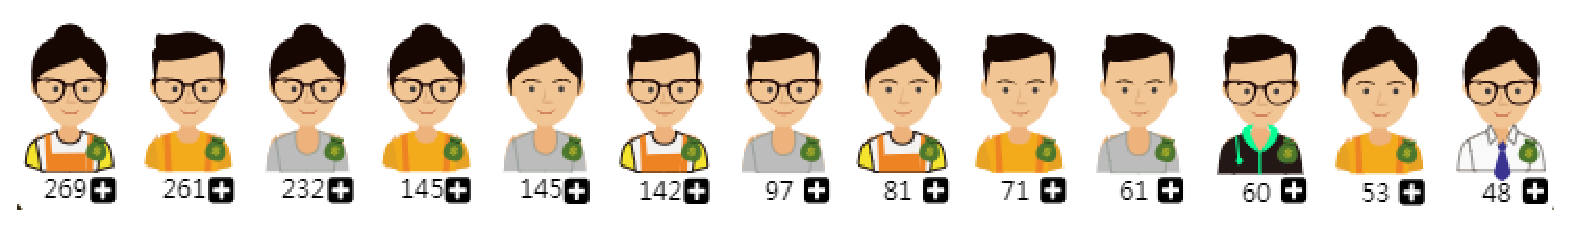
\includegraphics{pictures/case112.eps}}}\hspace{5pt}
% \subfigure[New rich.]{
% \resizebox*{4.4cm}{!}{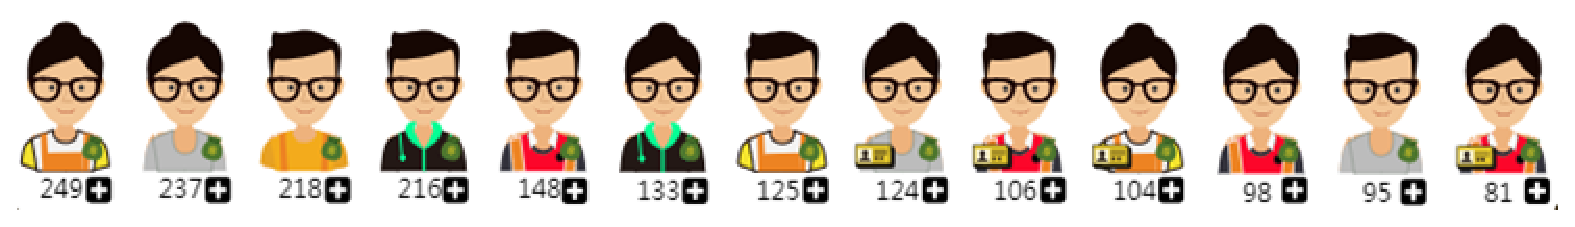
\includegraphics{pictures/case113.eps}}}\hspace{5pt}
% \subfigure[Antizen.]{
% \resizebox*{4.4cm}{!}{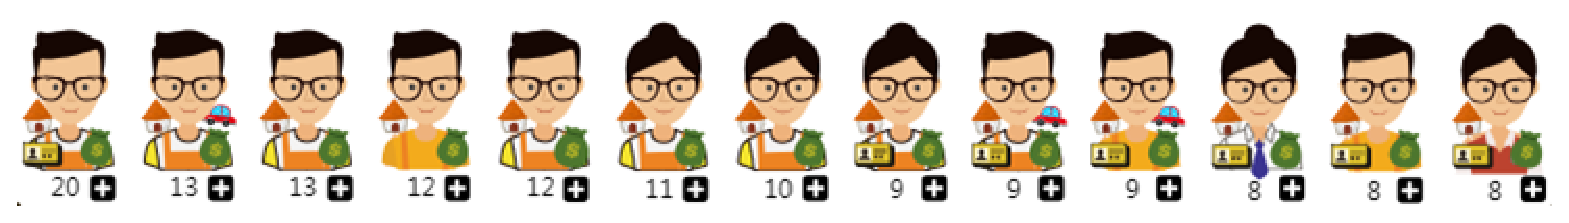
\includegraphics{pictures/case114.eps}}}\hspace{5pt}
% \caption{XXXXXX of different groups.}
% \label{case11}
% \end{figure}


% \begin{figure}
% \centering
% \subfigure[Top aristocracy.]{
% \resizebox*{4.4cm}{!}{
\includegraphics{pictures/case121.eps}}}\hspace{5pt}
% \subfigure[The underclass.]{
% \resizebox*{4.4cm}{!}{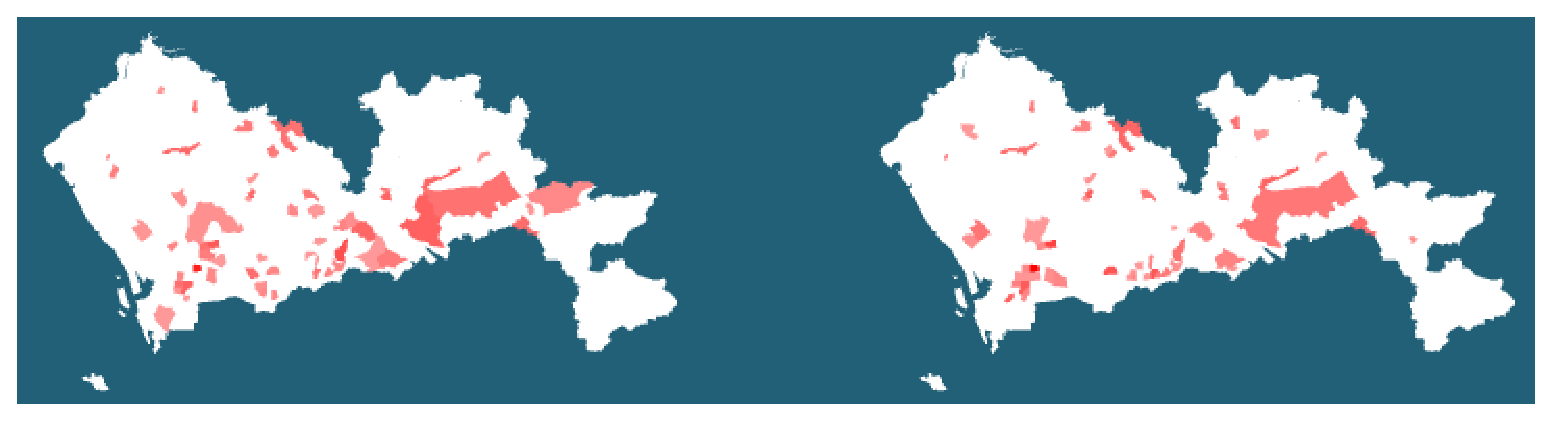
\includegraphics{pictures/case122.eps}}}\hspace{5pt}
% \subfigure[New rich.]{
% \resizebox*{4.4cm}{!}{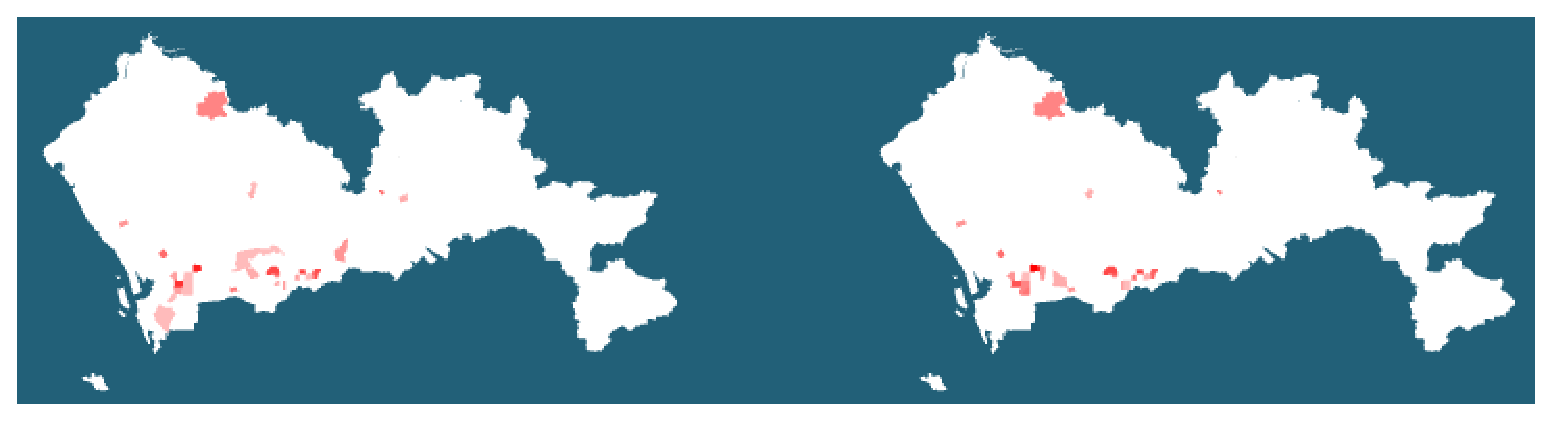
\includegraphics{pictures/case123.eps}}}\hspace{5pt}
% \subfigure[Antizen.]{
% \resizebox*{4.4cm}{!}{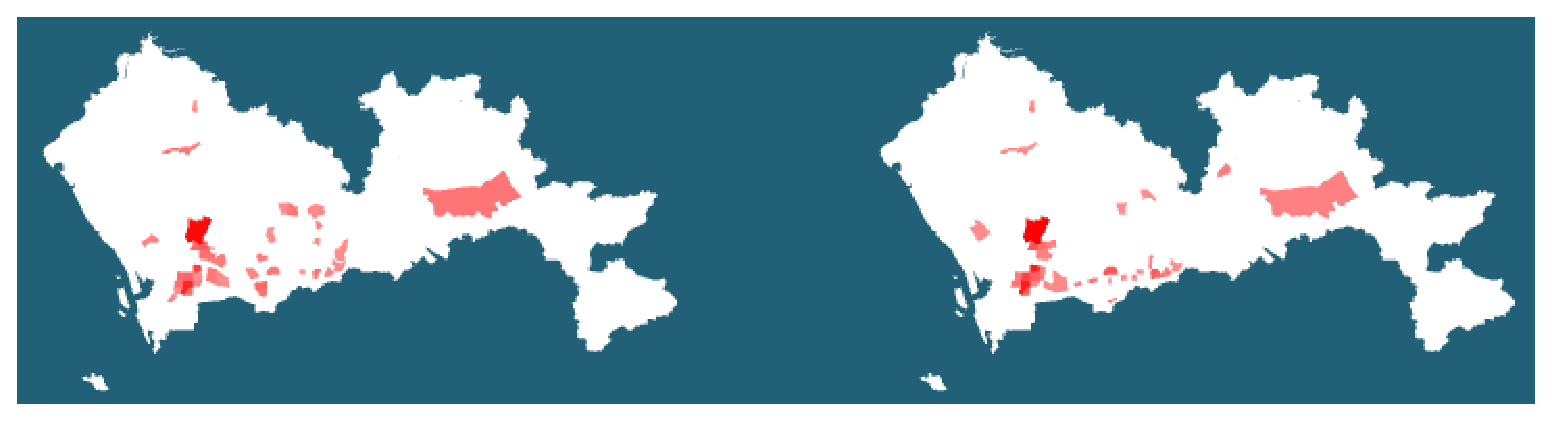
\includegraphics{pictures/case124.eps}}}\hspace{5pt}
% \caption{}
% \label{case12}
% \end{figure}


This work is inspired and motivated by the implication in science fiction~\textit{Folding Beijing}, which is that people are categorized into three classes and behave in the parallel spatial-temporal patterns. The first cast explores whether the folding city exists in reality or not.

\begin{figure}[htb!]
 \centering % avoid the use of \begin{center}...\end{center} and use \centering instead (more compact)
 \includegraphics[width=\columnwidth]{pictures/case1_1}
 \caption{Four Groups Divided by Income and Education Characteristics}
 \label{case11}
\end{figure}

Although it is incomplete, income and education are two of the most essential characteristics to tag an individual with a good resource or not. 
As Figure~\ref{case11} shows, taking income and education as the two dimensions, taking 300K yuan as the border between high and low income and an undergraduate bachelor degree as the border between high and low education level, four different groups are generated in the four quadrants. In the first quadrant, individuals are rich and well educated, who are in a group of so-called \textit{top aristocracy}. The second quadrant holds the group of \textit{new rich}, i.e., individuals with high income but low education income. In the third quadrant, they are the \textit{underclass} who has both low income and education level. The fourth quadrant is \textit{Antizen}, which is a new word to describe people have a good education but earn little. 


Figure~\ref{case11} shows the top 12 profiles with the maximum population in each group. In each group, other characteristics surprisingly demonstrate the high correlation to income and education. For example, almost all of the \textit{top aristocracy} is with the residential license,  house, and car. On the contrary, \textit{underclass} do not have the residential license residence, neither the house nor the car. Most of \textit{New rich} has a house and work in the service industry.  

Before diving into the complex mobility pattern analysis, we explore the home distribution of the four groups. As Figure~\ref{case12} shows, \textit{top aristocracy} and most of \textit{new rich} live concentrated in the downtown area of Shenzhen, where the living cost is higher, especially the housing cost. A small part of \textit{new rich} lives far away from the downtown, maybe because they don't have to work in downtown. The \textit{underclass} distribute more dispersively all over the whole city. Compared to the rich, they prefer the outer space because of the lower living cost. Lots of \textit{antizen} live in Nanshan District, where there are many universities and high-tech industrial parks full of well educated people. 

\begin{figure}[htb!]
 \centering % avoid the use of \begin{center}...\end{center} and use \centering instead (more compact)
 \includegraphics[width=\columnwidth]{pictures/case1_2}
 \caption{Home Distributions of the Four Groups}
 \label{case12}
\end{figure}


% To understand how citizens live in the city, there are two crucial aspects to be known: during the night where they sleep, and where do they do during the daytime. ``Home location" could answer the first question. The second one is harder to summarise because of the complexity of daytime activities. In our method, we divide daytime mobility activities into 

To have a better knowledge of mobility patterns of the four groups, trips are categorized into three categories, ``home", ``work'' for regular trips with the purpose of going home, work (or school for students), ``other'' for irregular trips with the purpose of shopping, visiting friends. Figure~\ref{case13}(a) shows the 2.5D overview of the three kinds of traveling categories. Each TAZ is grown to the same height, i.e., the unit one, and the height proportion of each traveling categories encodes the percentage of certain purpose in the whole, pink for ``others'', blue for ``work'' and green for ``home''. Although inside TAZ prisms are blocked in the Figure~\ref{case13}, our attention is drawn to the lifestyle of \textit{New Rich}. It is founded that the \textit{New Rich} travel for ``other'' purpose a lot, compared to other groups. To explore further, the detail slicing (introduced in Section~\ref{subsec:25D}) is applied to the four groups. Figure~\ref{case13}(b) shows three slices. It can be seen that individuals with low income (\textit{underclass} and \textit{antizen}) spend relatively more time on work, especially the \textit{underclass}. Working percentage is very small in-group \textit{new rich}. They live a more diverse lifestyle because they do many other things (the pink ones) except working.


\begin{figure}[htb!]
 \centering % avoid the use of \begin{center}...\end{center} and use \centering instead (more compact)
 \includegraphics[width=\columnwidth]{pictures/case1_3}
 \caption{Mobility Patterns of ``work", ``home" and ``not essential" of the Four Groups: (a) the overview of the three pecentage; (b) three slices for detailed comparison.}
 \label{case13}
\end{figure}

% By comparing them, it can be seen that the poor spend more time on work, especially ``the underclass". Working percentage is really small in-group ``new rich". They have diverse lives because they do many other things except for working.


% \begin{figure}
%   \centering
%   \includegraphics[width=0.95\linewidth]{pictures/case1_4}
%   \caption{Examples of XXXXX.}
%   \label{case14}
% \end{figure}
% two categories to capture mobility patterns. ``routine activity" is made up with ``go to work", ``go to school" and ``go back home". Movements with other purposes are ``not essential". People do these movement activities due to their personal willingness and living style. Therefore, ``home location", ``working location" and ``not essential" activity space outline one's living space. Our system meets this requirement.

% In Fig. \ref{case13}, the distributions of ``essential" activity including ``go to work" and ``go home", and ``not essential activity" are shown. 

% From the dimension of space, ``new rich" prefer to live in the west of the city. They do not go south-east in most times. Other three groups reach the whole city. The height of the bar stands for the percentage of each kind of activity. Higher height means that the group has more willingness and cost more time in ``, not the essential activity", while lower height means more time on work. As we described in Section XXX, �ڵ�����, ����ʹ���������� Fig. \ref{case14} give three examples within each group to check the detailed information in the 2.5D graph. By comparing them, it can be seen that the poor spend more time on work, especially ``the underclass". Working percentage is really small in-group ``new rich". They have diverse lives because they do many other things except for working.


\subsection{Case 2: Home-work Distance VS Income/House}


\begin{figure}[htb!]
 \centering % avoid the use of \begin{center}...\end{center} and use \centering instead (more compact)
 \includegraphics[width=\columnwidth]{pictures/case2}
 \caption{Home-work distances of different groups: (a) with different salary levels; (b) with or without house.}
 \label{case2}
\end{figure}

% \begin{figure}
% \centering
% \subfigure[Group of people whose income more than 500,000yuan per year.]{
% \resizebox*{4.4cm}{!}{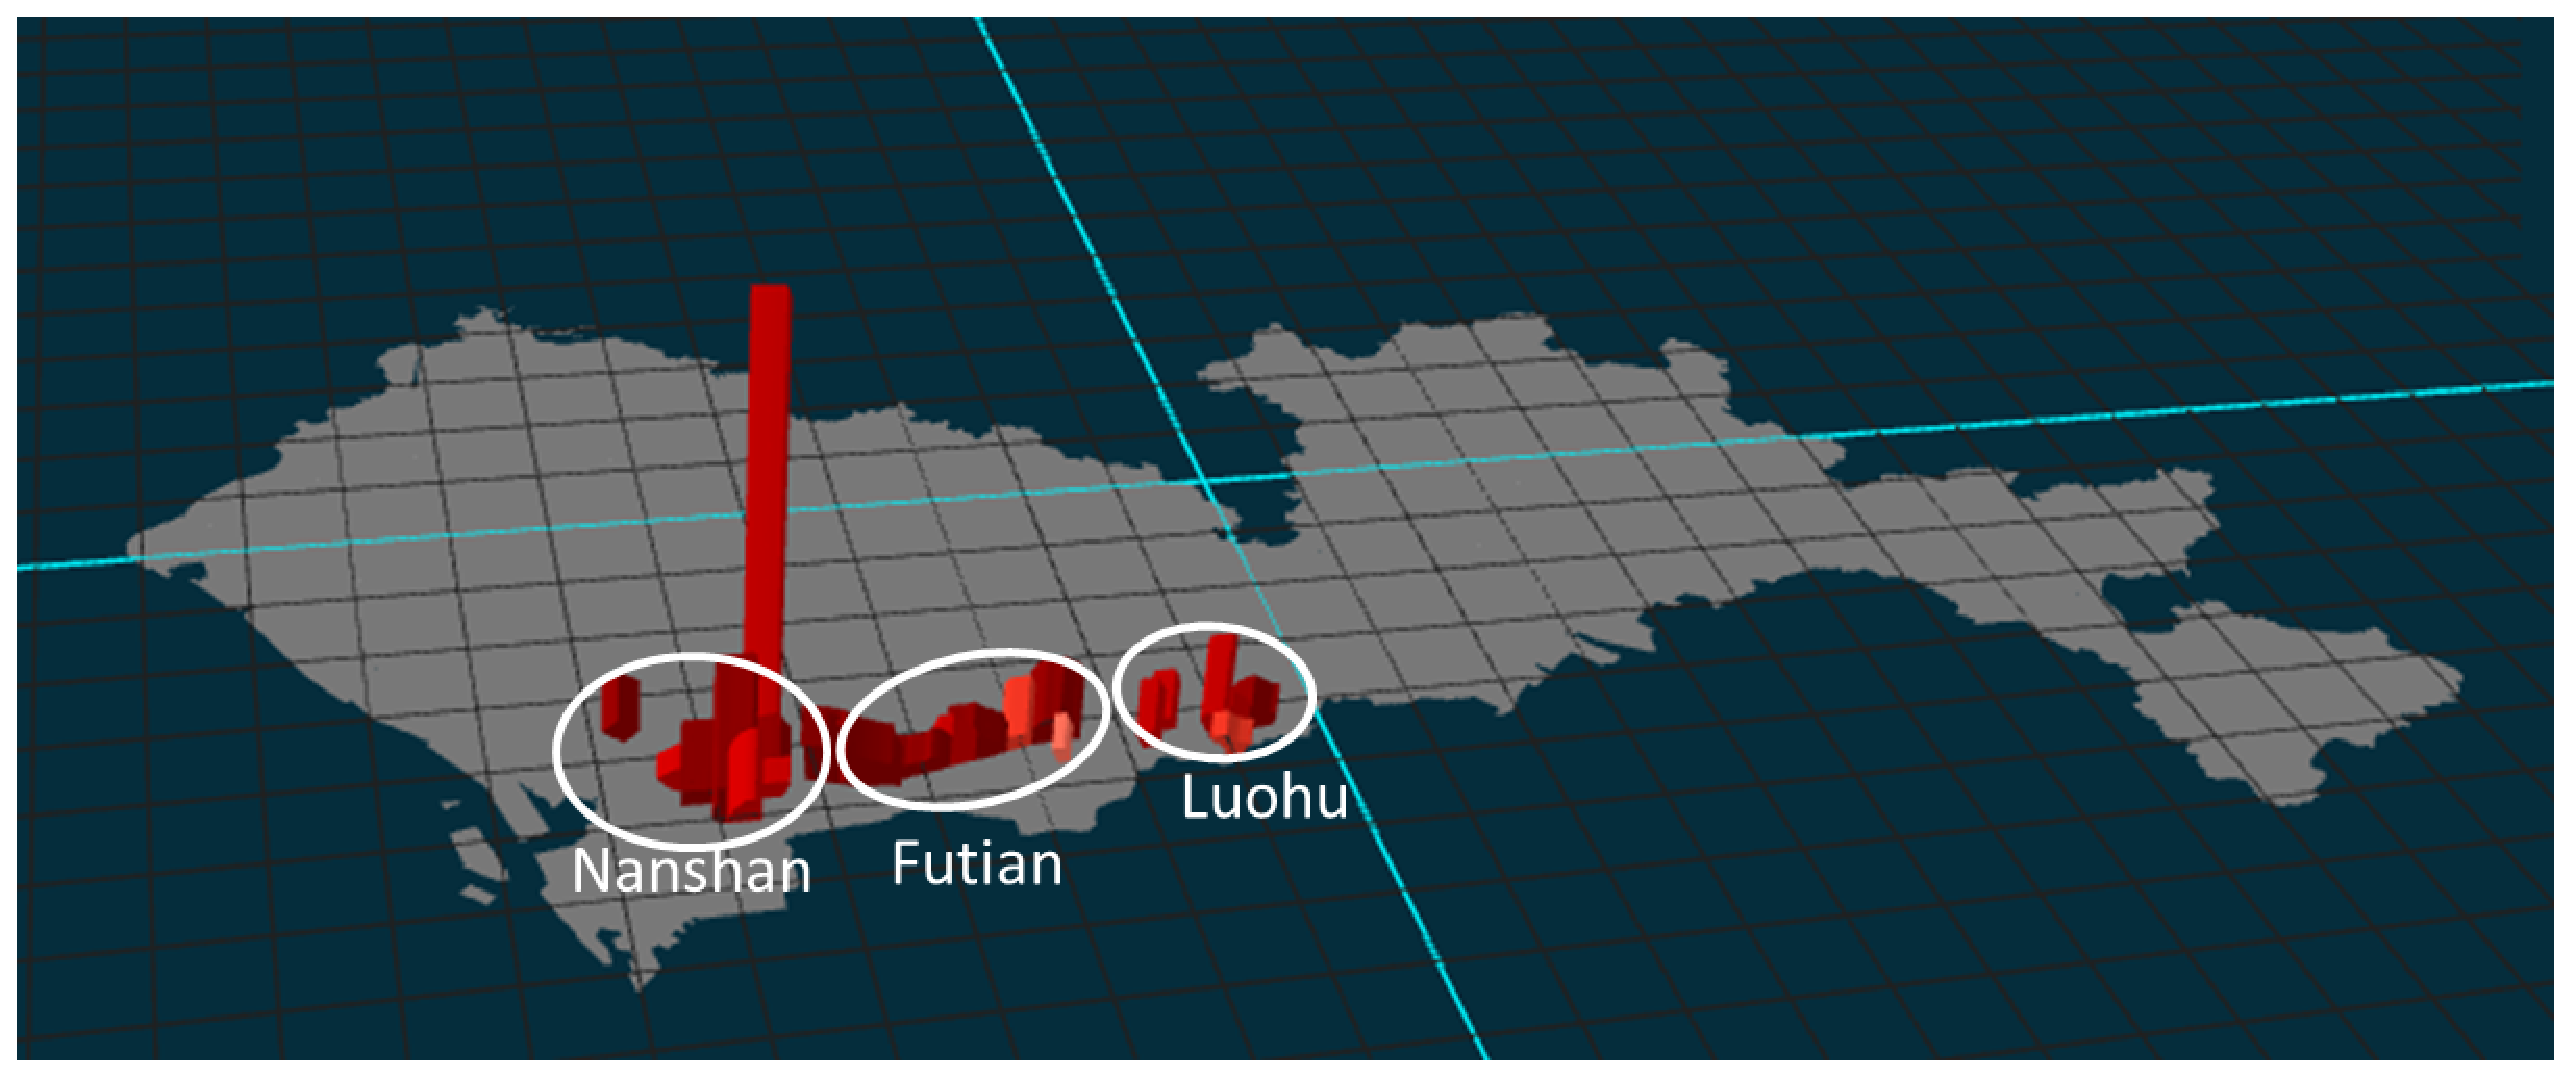
\includegraphics{pictures/case21.eps}}}\hspace{5pt}
% \subfigure[Group of people whose income between 200,000 yuan to 300,000 yuan per year.]{
% \resizebox*{4.4cm}{!}{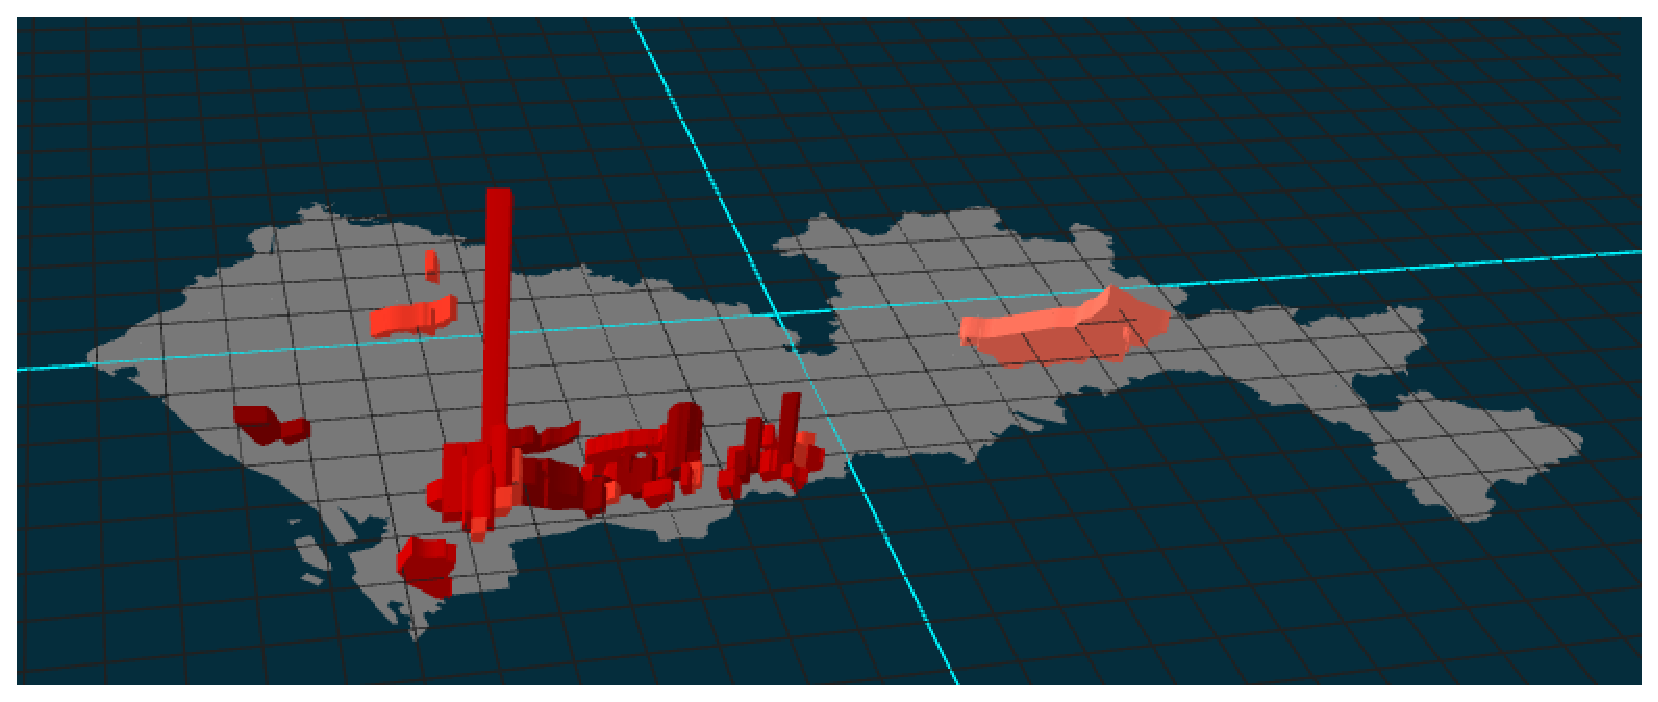
\includegraphics{pictures/case22.eps}}}\hspace{5pt}
% \subfigure[Group of people whose income less than 100,000yuan per year.]{
% \resizebox*{4.4cm}{!}{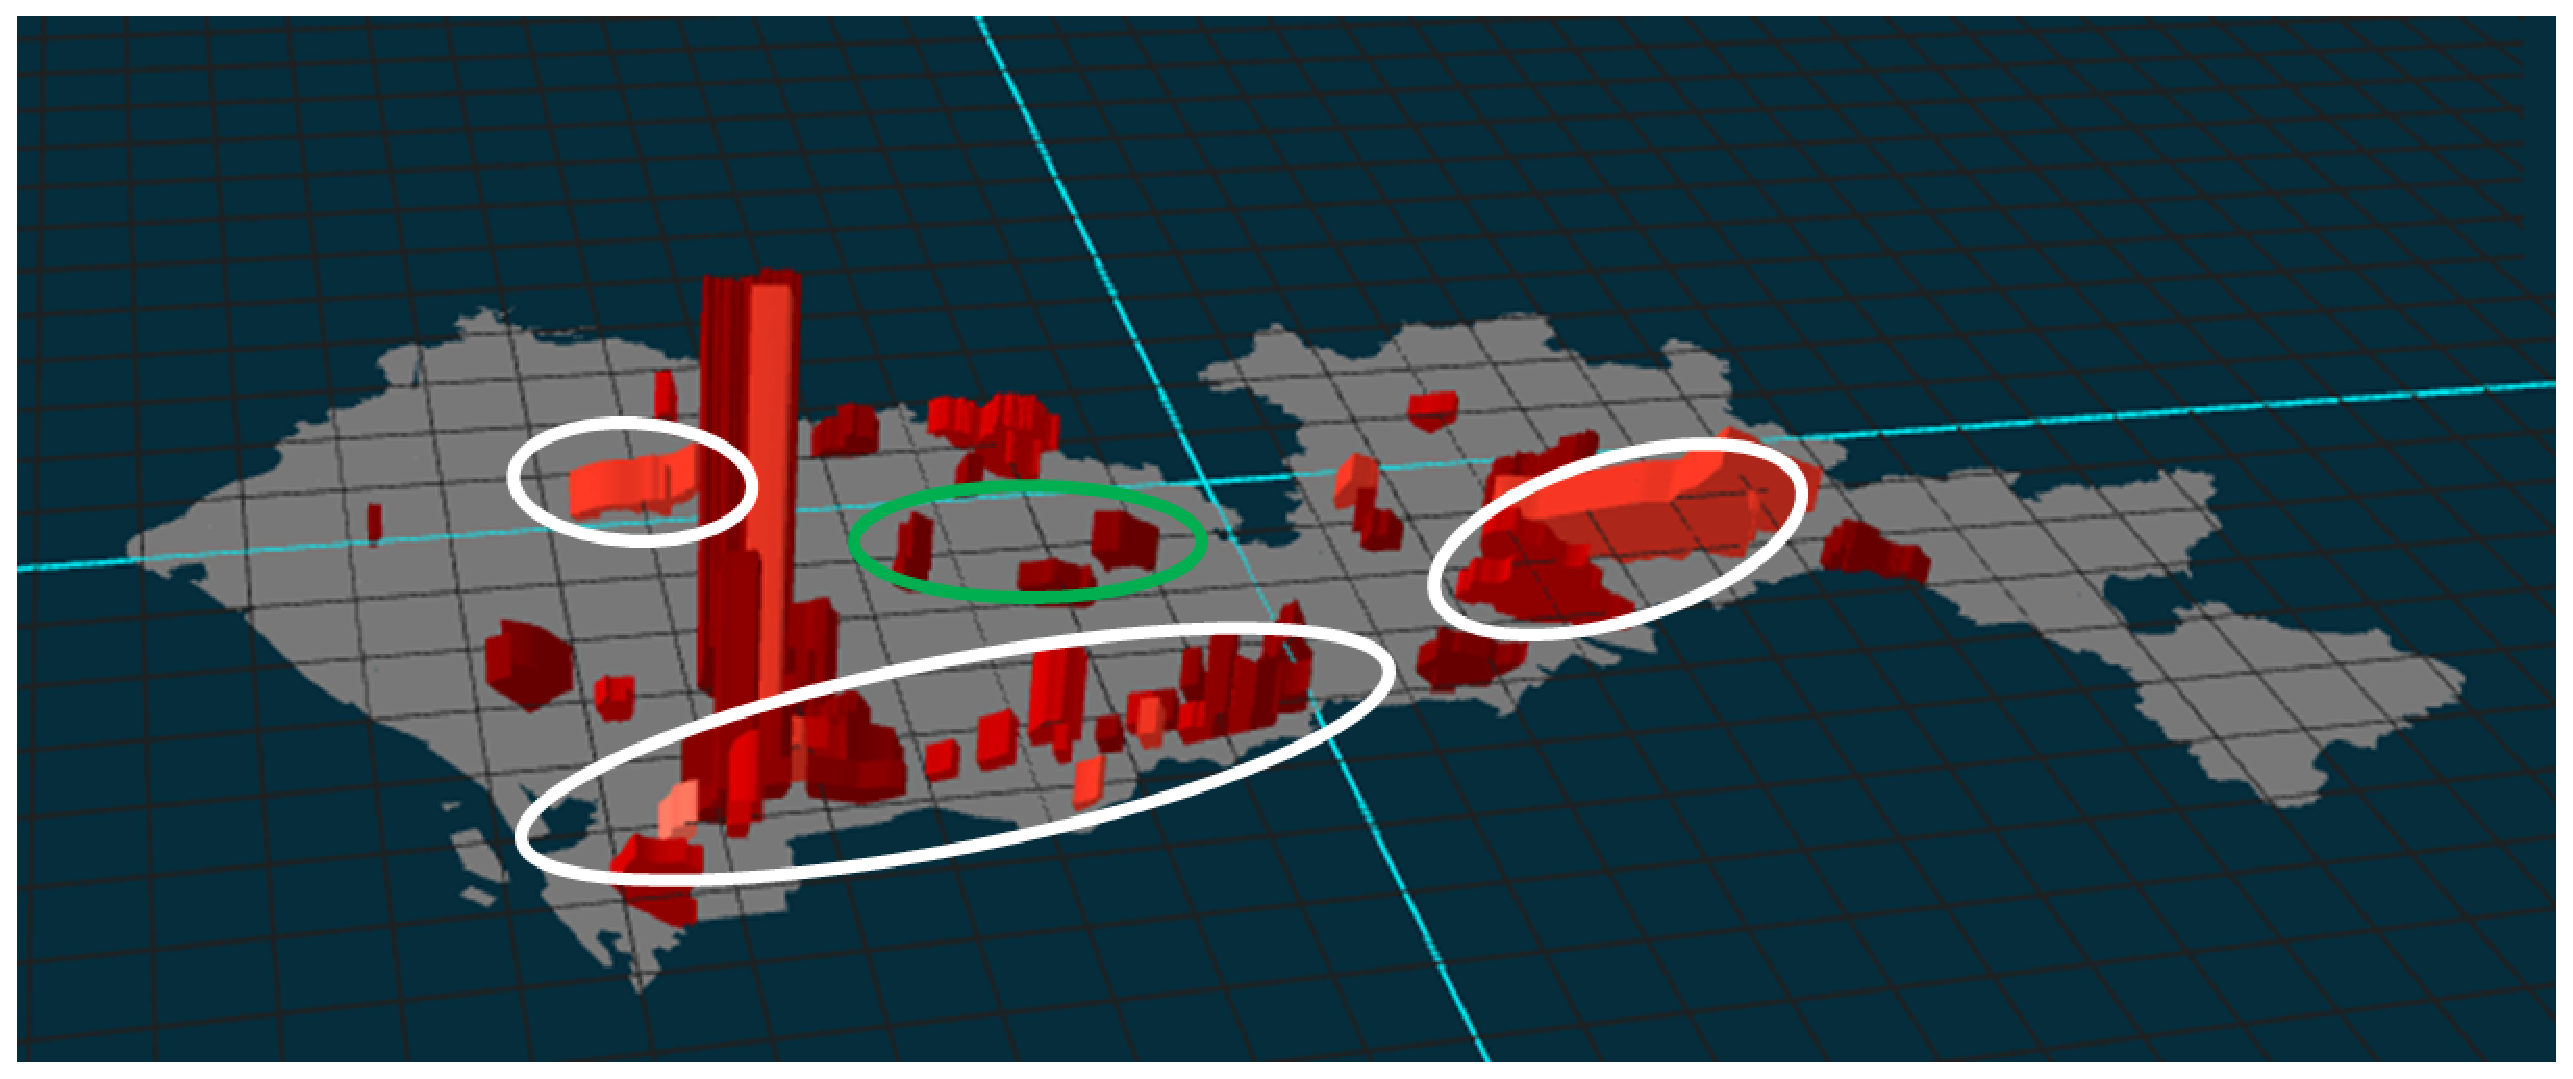
\includegraphics{pictures/case23.eps}}}\hspace{5pt}
% \subfigure[Group of people who owe house.]{
% \resizebox*{4.4cm}{!}{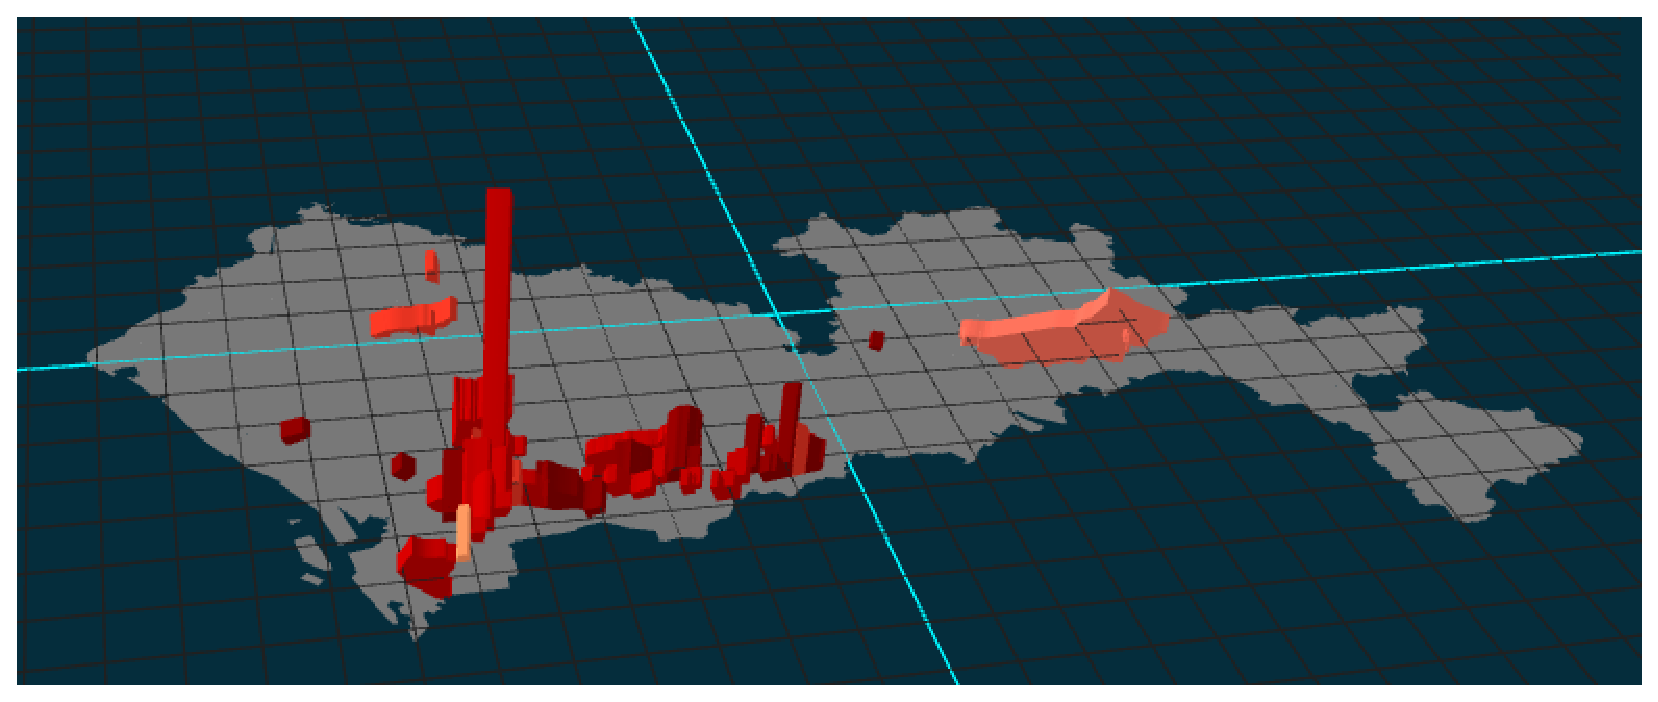
\includegraphics{pictures/case24.eps}}}\hspace{5pt}
% \subfigure[Group of people who rent house.]{
% \resizebox*{4.4cm}{!}{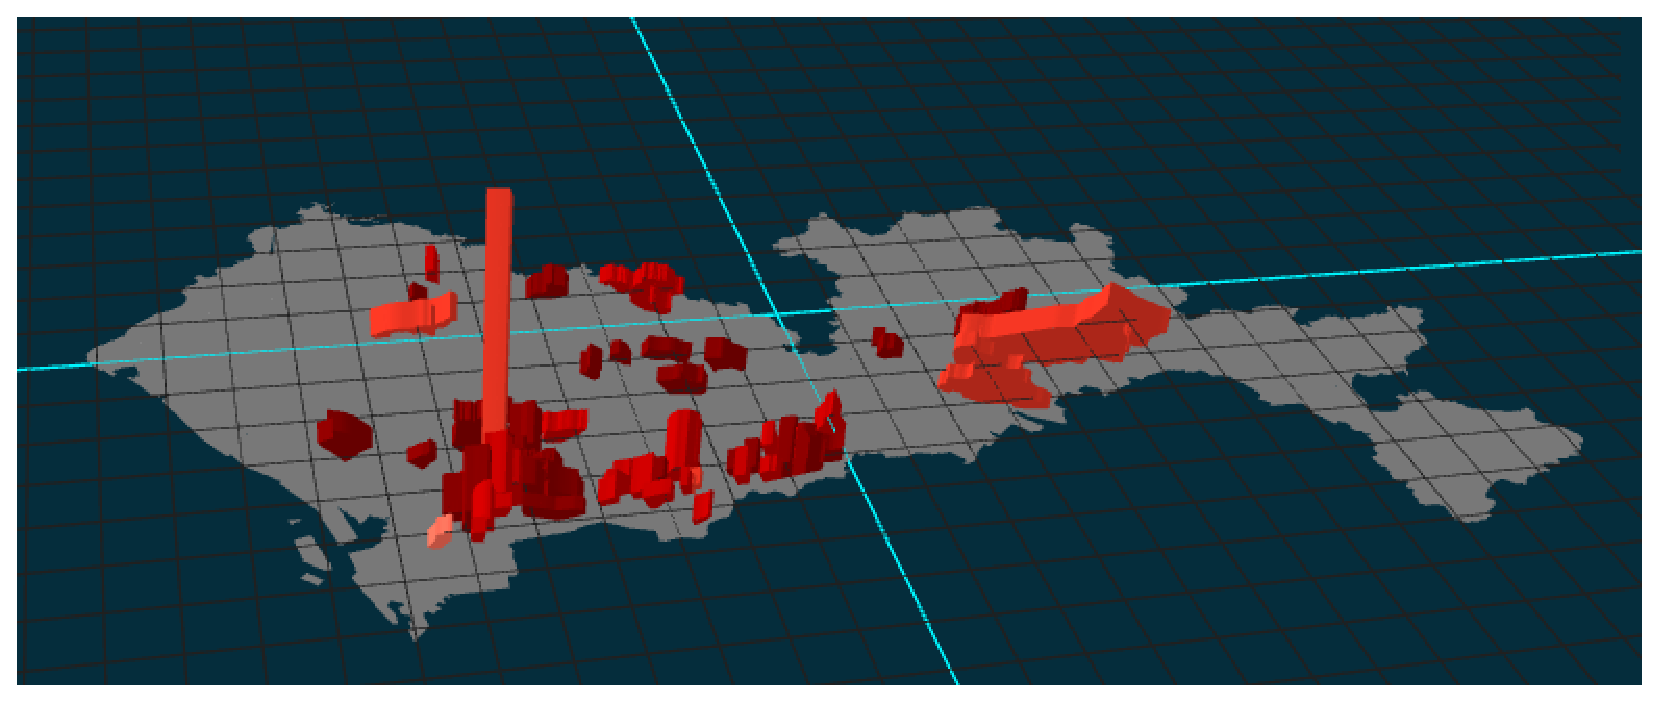
\includegraphics{pictures/case25.eps}}}\hspace{5pt}
% \caption{Home-work distances of different groups.}
% \label{case2}
% \end{figure}

Home-work distance is an essential metric in economics, geography, and sociology. It refers to the distance between house and workplace. It is influenced by many factors like transportation, housing, land use, etc. Understanding the home-work distance of a region helps to evaluate whether the region is well planned or not. In this case, we demonstrate our system's help in home-work distance understanding.

Considering income potentially determines where people live, we use income as the characteristics to select three groups, the group over 500K, the group during 200-300K and the group less than 100K. In Figure~\ref{case2}, the height of the bar stands for visiting frequency of the TAZ and its color encodes the average home-work distance, red for close and yellow for far. As Figure~\ref{case2}(a) shows, for all the three groups in different income levels, most of the TAZs have dark red or red color which indicates the home-work distance is generally short, especially in downtown. Only those with less than 100K salary work outside the center, such as the space in the green circle. When comparing the three groups in the downtown area, it is seen that it takes more time to go to work in Futian District as the decrease of the income. 

We explore the home-work distance of groups with and without a house. 
Figure~\ref{case2}(b) shows the close-up views. It is found that the Nanshan District has a shorter home-work distance for individuals without a house, while Futian District has shorter for those with a house. Nanshan is relatively newer to Futian so that there might be more easily-accessible houses to be rent.

  % District belongs to all but Futian District belongs to the rich. The poor could rent house living in Nanshan and Luohu to enjoy short home-work distance. In Futian, only the rich working there have short home-work distance. There may be no much housing for rent.

 % From the figure, it is seen that the working locations are mainly in three areas which are circled in white in Fig. \ref{case2}(c). Space in green circle is another hot working area which only is preferred by the poor.
% On the whole, home-work distance is short in Shenzhen for most of the TAZs with different groups have a darker color, especially in downtown. When focusing on the downtown area, it is seen that there are differences between Futian District with the other two. By comparing three groups distinguished by income, it takes more time to work in Futian District with the decrease of the income. Meanwhile, the opposite is true in others. In combination with Fig. \ref{case2}(d) and Fig. \ref{case2}(e), 


\subsection{Case 3: Life-style VS Jobs}

% \begin{figure}
% \centering
% \subfigure[Officer.]{
% \resizebox*{4.4cm}{!}{\includegraphics{pictures/311.eps}}}\hspace{5pt}
% \subfigure[Workman.]{
% \resizebox*{4.4cm}{!}{\includegraphics{pictures/321.eps}}}\hspace{5pt}
% \subfigure[Student.]{
% \resizebox*{4.4cm}{!}{\includegraphics{pictures/331.eps}}}\hspace{5pt}
% \subfigure[Businessman.]{
% \resizebox*{4.4cm}{!}{\includegraphics{pictures/341.eps}}}\hspace{5pt}
% \caption{Percentage of movement with purposes in group of different jobs.}
% \label{case31}
% \end{figure}

In this case, we explore the correlation between mobility patterns with the job, to see whether the job has an impact on the movement. Officer, workman, student, and businessman are selected as examples and the population of trips for certain purposes is shown In Figure~\ref{case3}. The height of bars encodes the amount of visit to each TAZ, and color encodes the traveling purpose. There are 10 different kinds of traveling purposes. For quick linking between color and purposes, the regular trips such as go to work, school and home are dyed in cold color, and the irregular trips such as go shopping, hospital, etc, are dyed in the warm color. As Figure~\ref{case3} shows, for officers, the TAZs changes dramatically in height. Some TAZs have much more visiting than others because officers are more constrained to work in some buildings than individuals with other jobs. The relative percentage of irregular activity differs for the four groups. For Workman, about 80 percent of movements are the regular purpose, either go to work or go back home. For students, the percentage becomes to be about 50 percentage. Compared to them, officer and businessman have more flexible and diversified lifestyle.




% Each social attribute has an impact on movement patterns. There are 9 kinds of jobs in the data which offers rich information. Therefore, in this case, we use ``job" as the target social attribute to explore its influence on citizens' movement patterns.

% At first, with 2.5D spatial visual form, we learn what people move for and the percentage of movements with a given purpose. 

% The height of each bar stands for the number of movements to the TAZ. Purposes are encoded in color as the legends show. From the perspective of the height of bars, it is seen that the amount of visitors to each TAZ of officers is really different. Several TAZs have the dominant visiting. In Figure~\ref{case3}(a), the heights of yellow bars and rose red bars in different TAZs have great differed. This phenomenon is not that obvious in other three groups. In addition, the percentage of ``not essential" activity differs. For Workman, about 80 percent of movements are ``essential" ones. For students, the percentage becomes to be about 50 percentage. Compared to them, officer and businessman have more flexible and diversified lives.


\begin{figure}[htb!]
 \centering % avoid the use of \begin{center}...\end{center} and use \centering instead (more compact)
 \includegraphics[width=\columnwidth]{pictures/case3}
 \caption{Trip purposes distribution of four groups with different jobs}
 \label{case3}
\end{figure}

Next, we concentrated on one purpose to see whether it is related to jobs. Here we use ``dinner or entertainment" as the example. As Fig \ref{case32} shows, the height of TAZ bars represents the visiting amount of trips for dinner or entertainment. Color stands for moving distance to reach this TAZ. As we can see, officers prefer to entertain in the downtown area, while workmen cover a larger area. Students tend to concentrate on Nanshan district, probably near schools. For the businessmen, they go lots of places for dinner or entertainment. The biggest difference with other groups is that they would travel a long distance to go somewhere far from downtown areas. 

\begin{figure}[htb!]
 \centering % avoid the use of \begin{center}...\end{center} and use \centering instead (more compact)
 \includegraphics[width=\columnwidth]{pictures/case3_2}
 \caption{The ``dinner or entertain" purpose of four groups with different jobs}
 \label{case32}
\end{figure}

% \begin{figure}
% \centering
% \subfigure[Officer.]{
% \resizebox*{4.4cm}{!}{\includegraphics{pictures/314.eps}}}\hspace{5pt}
% \subfigure[Workman.]{
% \resizebox*{4.4cm}{!}{\includegraphics{pictures/324.eps}}}\hspace{5pt}
% \subfigure[Student.]{
% \resizebox*{4.4cm}{!}{\includegraphics{pictures/334.eps}}}\hspace{5pt}
% \subfigure[Businessman.]{
% \resizebox*{4.4cm}{!}{\includegraphics{pictures/344.eps}}}\hspace{5pt}
% \caption{}
% \label{case32}
% \end{figure}



\section{Conclusion}
\label{sec:conclusion}

Combined travel demands, this work illustrates the relationship between accessibility and behaviour within the region, which in turn can be used to forecast the traveling trips. 

derive zonal level analysis thich can be used in transportation applications.

Our analysis demonstrates how demographics survey collectd via social media have the potential to indiate the movement patterns of groups that have different social charactersitics and the difference in using urban facilities. Better understand of the interactions between population characteristics and their urban activity. The data we used represent a small propotion of the population of which we do not have the clear definition of its demographics. We consider this work as one of the first steps of research contextualize the analysis of urban dynamcis with social science, to understand the  interactions between population characteristics and their urban activity. 

\bibliographystyle{abbrv}
%%use following if all content of bibtex file should be shown
%\nocite{*}
\bibliography{main}
\end{document}
